\documentclass[border = 120pt]{standalone}

\usepackage[landscape]{geometry}
\usepackage{tikz}
% \usetikzlibrary{mindmap}
% \usepackage{metalogo}
\usetikzlibrary{shapes, snakes}
\begin{document}
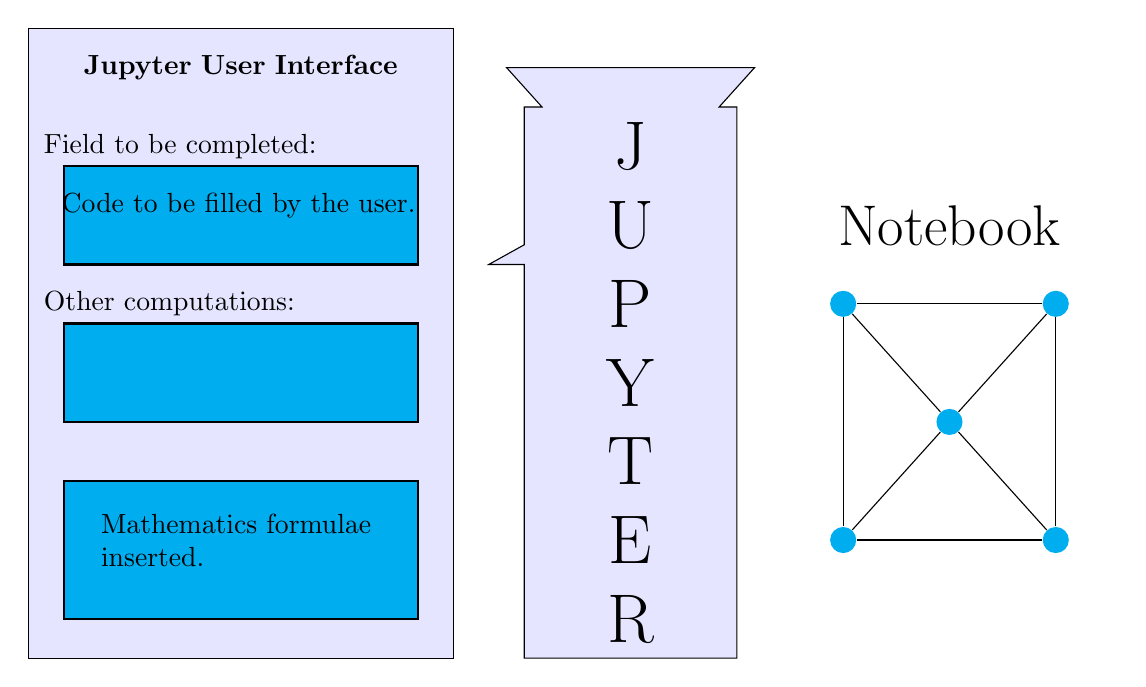
\begin{tikzpicture}[xscale=.9]

%Mother Ship
\draw[fill=blue!10] (-7,-3.5) rectangle (-13, 4.5);

%Jupyter Interface
\node[align=center, text width=5cm] at (-10,4) {\textbf{Jupyter User Interface}};
\node[align=left, text width=5cm] at (-10,3) {Field to be completed:};

%% User Interface
\draw[style=thick, fill=cyan] (-12.5, 2.75) rectangle (-7.5, 1.5);
\node[align=left, text width=5cm] at (-9.75,2.25) {Code to be filled by the user.};
\node[align=left, text width=5cm] at (-10,1) {Other computations:};
\draw[style=thick, fill=cyan] (-12.5, 0.75) rectangle (-7.5, -0.5);

\draw[style=thick, fill=cyan] (-12.5, -1.25) rectangle (-7.5, -3);
\node[align=left, text width=4cm] at (-9.75,-2) {Mathematics formulae inserted.};

% First machine
\path[draw, fill=blue!10] 
(-6, -3.5) -- 
(-6, 1.5) -- 
(-6.5, 1.5) -- 
(-6, 1.75) -- 
(-6, 3.5) -- 
(-5.75, 3.5) -- 
(-6.25, 4) -- 
(-2.75, 4) --
(-3.25, 3.5) -- 
(-3, 3.5) -- 
(-3, -3.5) -- 
cycle;

\node at (-4.5, 3) {\Huge J};
\node at (-4.5, 2) {\Huge U};
\node at (-4.5, 1) {\Huge P};
\node at (-4.5, 0) {\Huge Y};
\node at (-4.5, -1) {\Huge T};
\node at (-4.5, -2) {\Huge E};
\node at (-4.5, -3) {\Huge R};

\tikzstyle{every node} = [circle]
\node[fill=cyan] (a) at (-1.5, -2) { };
\node[fill=cyan] (b) at (1.5, -2) { };
\node[fill=cyan] (c) at (1.5, 1) { };
\node[fill=cyan] (d) at (-1.5, 1) { };
\node[fill=cyan] (e) at (0, -0.5) { };
\foreach \from/\to in {a/b, b/c, c/d, a/d, a/e, e/b, c/e, d/e}
\draw [-] (\from) -- (\to);

\node[align=center, text width=4cm] at (0,2) {\huge Notebook};

\end{tikzpicture}
\end{document}

%%% Local Variables:
%%% mode: latex
%%% TeX-master: t
%%% End:
